\section{Entscheidungsprozesse}

\begin{frame}[c]{Fehlerquellen in Entscheidungsprozessen}
    \centering
    % Folie langsam aufbauen, ist sonst zu viel information auf einmal
    % Konkretes Beispiel!!
    % ideen: Kaufen eines Produktes im Supermarkt
    % idee: Terminoptimierung - Freizeitoption A oder B, fokus auf Gruppendynamik
    \only<1>{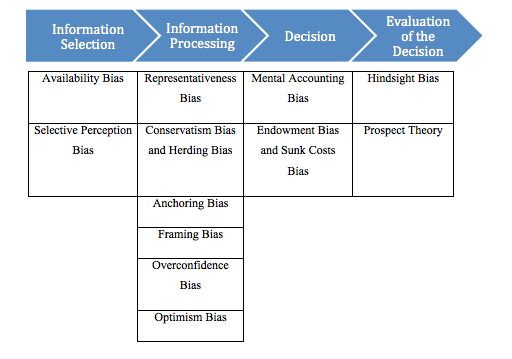
\includegraphics[width=\textwidth, clip=true, trim= 0mm 102mm 0mm 0mm]{DecisionMakingProcedure}}
    \only<2>{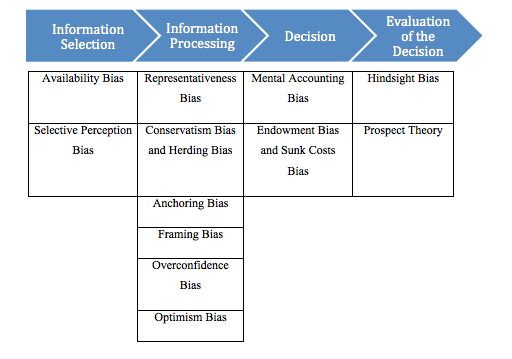
\includegraphics[width=\textwidth]{DecisionMakingProcedure}}
\end{frame}


\begin{frame}[standout]
    ... und das ist nur ein kleiner Auszug.
\end{frame}

\begin{frame}[c]{List of cognitive Biases}
    \centering
    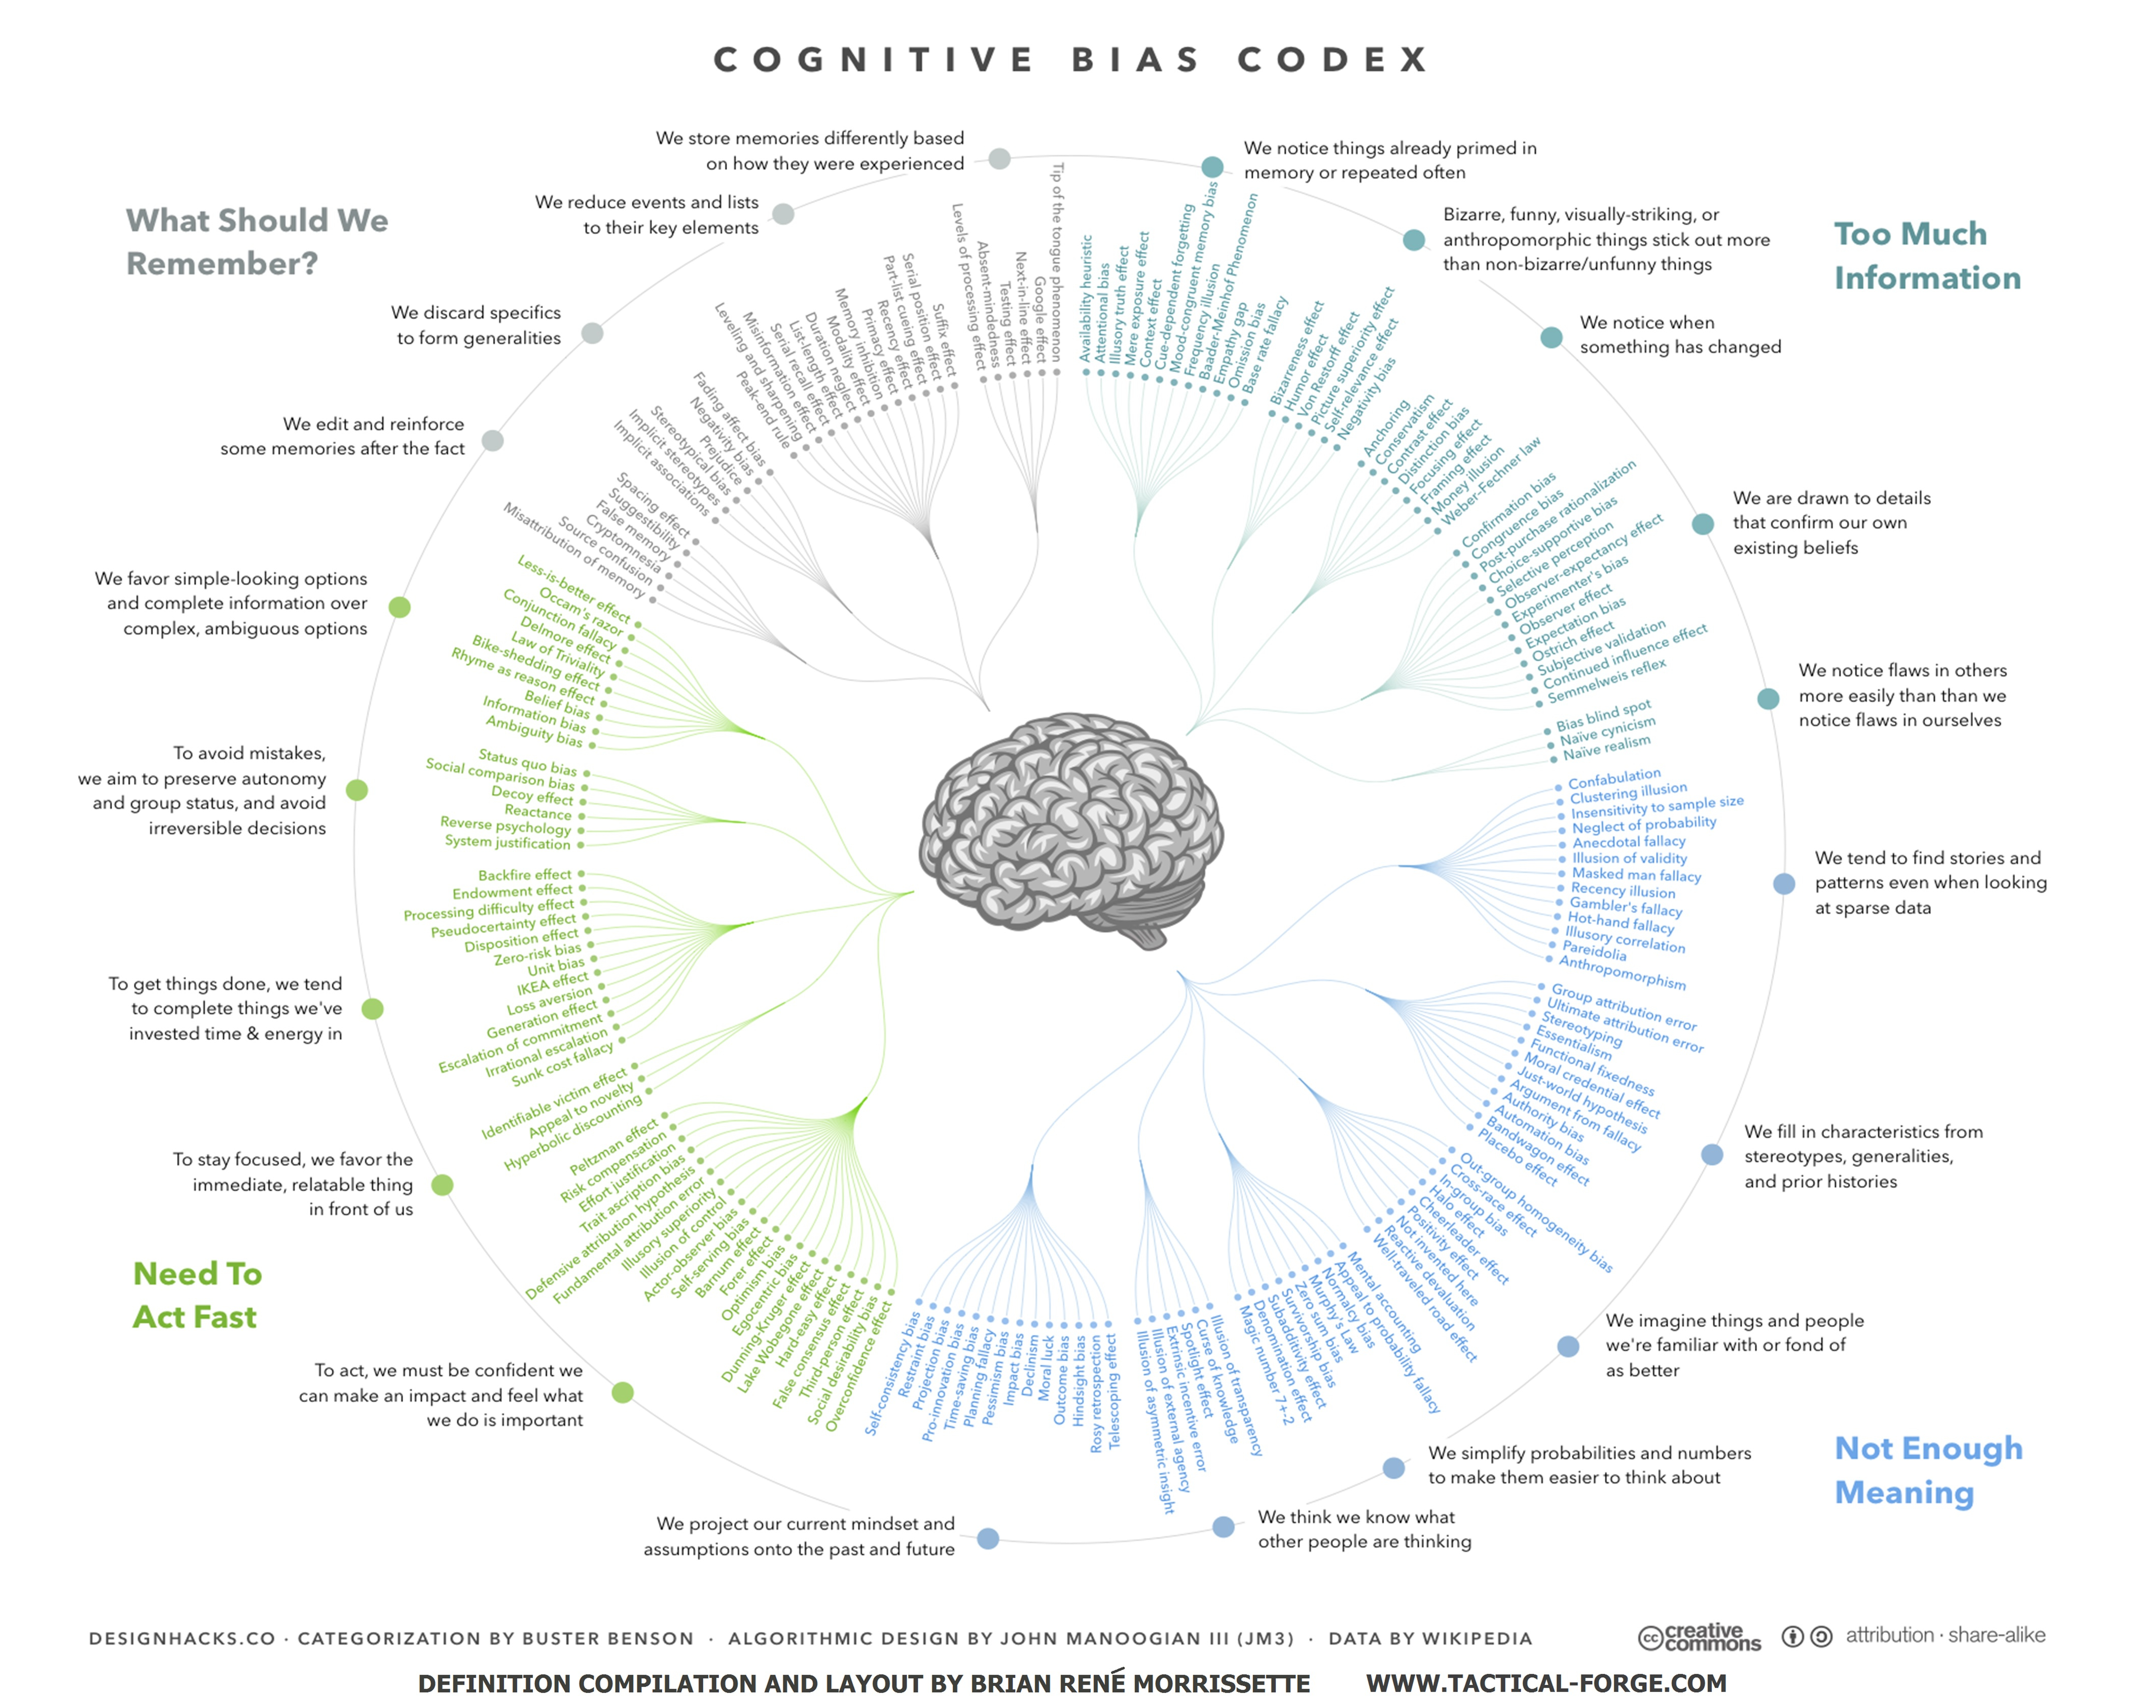
\includegraphics[width=\textwidth]{cogbias_0}
\end{frame}


\begin{frame}[c]{Denken, schnell und langsam}
    \Large
    \pause
    % Das Gehirn arbeitet üblicherweise mit zwei verschiedenen Systemen
    \begin{itemize}
    \item System I - schnelles Denken
    \newline
    \pause
    \item System II - langsames Denken
    \end{itemize}
\end{frame}

